%% Use the option review to obtain double line spacing
%% \documentclass[authoryear,preprint,review,12pt]{elsarticle}

%% Use the options 1p,twocolumn; 3p; 3p,twocolumn; 5p; or 5p,twocolumn
%% for a journal layout:
%% \documentclass[final,1p,times,authoryear]{elsarticle}
%% \documentclass[final,1p,times,twocolumn,authoryear]{elsarticle}
%% \documentclass[final,3p,times,authoryear]{elsarticle}
%% \documentclass[final,3p,times,twocolumn,authoryear]{elsarticle}
%% \documentclass[final,5p,times,authoryear]{elsarticle}
\documentclass[final,5p,authoryear]{elsarticle}
%% For including figures, graphicx.sty has been loaded in
%% elsarticle.cls. If you prefer to use the old commands
\usepackage{amssymb}
%% The amsthm package provides extended theorem environments
%% \usepackage{amsthm}
\usepackage{lineno}
\usepackage{booktabs}
% ---------------------------------------------------------------------
%             FOR DRAFTING / REVIEW (DELETE BEFORE SUBMISSION)
% ---------------------------------------------------------------------
\usepackage{caption}
\usepackage{subcaption}
\usepackage[T1]{fontenc}
\usepackage[british]{babel}
\usepackage{microtype}
\usepackage[tt=false]{libertine}
\usepackage{xcolor}
\definecolor{blue}{RGB}{33,150,209}
\definecolor{red}{RGB}{255,0,0}
\usepackage{xurl}
\usepackage[colorlinks=true, allcolors=blue]{hyperref}
\usepackage{pdfpages}
\usepackage{enumitem}
\usepackage{lineno}
\usepackage{float}
\setlength{\linenumbersep}{5pt}
% Save the old \texttt command
\let\oldtexttt\texttt
% Redefine the \UrlFont to use a smaller typewriter font
\renewcommand{\UrlFont}{\ttfamily\small}
% Redefine the \texttt command to use a smaller font size and allow line breaks
\renewcommand{\texttt}[1]{{\ttfamily\small\nolinkurl{#1}}}

\usepackage{tcolorbox}
\newcommand{\cbox}[1]{
    \begin{tcolorbox}[hbox, colback=red!5!white, colframe=red!65!black, boxrule=0.25pt, boxsep=2pt, left=2pt, right=2pt, top=1pt, bottom=1pt]
        \small\sffamily #1
    \end{tcolorbox}
}

% ------------------------------------------------------

\journal{Resources, Conservation and Recycling}

\begin{document}


\linenumbers

    % SPOTLIGHTS (5 bullet points, max 120 characters each)
    {\Large Spotlights}
    \vspace{1em}
    \begin{description}[style=nextline]
        \item[Bullet 1: Critical context and background information on the problem addressed] Tracking waste and material flows is essential for developing the circular economy and supply chain resilience
        \item[Bullet 2: A brief overview of the key finding of the study (or findings if necessary)] A tool was developed to quantify waste and material footprints of activities in life cycle assessment (LCA) databases
        \item[Bullet 3: The most radical, creative, disruptive or innovative aspect of the manuscript] Built to complement the Brightway LCA framework and ActivityBrowser, the tool is customisable and easy to use.
        \item[Bullet 4: The significance of the results to the environment, economics or society] The tool can be used to identify pre-consumer waste and material hotspots that are often hidden in supply chains.
        \item[Bullet 5: Future vision or the most important implications for continued research] Improved data availability and quality would enable more detailed and accurate waste and material footprinting.
    \end{description}

    \newpage
    %% GRAPHICAL ABSTRACT
    \begin{graphicalabstract}
        \includegraphics{grabs}
    \end{graphicalabstract}

    %% RESEARCH HIGHLIGHTS (3-5 bullet points, max 85 characters each)
    \begin{highlights}
        \item T-reX, a new tool for quantifying waste and material flows in LCA.
        \item Assesses supply risks by calculating demand for critical materials.
        \item Simplifies quantification of user-specified waste and material categories.
        \item Rapidly identifies waste and material demand hotspots.
        \item Presents a case study of the battery supply chain.
    \end{highlights}


\begin{frontmatter}

    \title{T-reX: A python package to quantify supply chain flows of waste and material in LCA databases}
    \author[1]{Stewart Charles McDowall\corref{cor1}}
    \ead{s.c.mcdowall@cml.leidenuniv.nl}
    \author[1]{Elizabeth Lanphear}
    \author[1]{Stefano Cucurachi}
    \author[1]{Carlos Felipe Blanco}

    \cortext[cor1]{Corresponding author:}

    \affiliation[1]{
        organization={Institute of Environmental Sciences (CML), Leiden University},
        addressline={P.O. Box 9518},
        city={Leiden},
        postcode={2300 RA},
        state={South Holland},
        country={The Netherlands}}

    \begin{abstract}
        \cbox{Abstract word count: 164, Limit: 150}
        Minimising waste through the reuse of resources is the quintessential principle of the `circular economy', but relies on our ability to identify and quantify waste and material flows.
        Thus, identifying and quantifying waste and material flows are of fundamental importance. Life Cycle Assessment (LCA) is powerful for this end, given its capacity to pinpoint hotspots of environmental impact throughout the life cycle of products and services, those where the implementation of circular principles could be most effective.

        Introducing T-reX, a Python tool extending the Brightway framework for flexible quantification of user-defined supply-chain demands in current and future scenarios. This tool streamlines database manipulation for LCA practitioners and integrates methods to aggregate and analyse waste and material flows, facilitating rapid hotspot identification.

        A case study on battery supply chains demonstrates the tool's utility. T-reX quantifies and compares inventory demands and, thus, potential environmental burdens, aiding sustainable decision-making. It contributes to the development of the `circular economy' by providing detailed material usage and waste generation analysis.

    \end{abstract}


    % KEYWORDS (max 6)
    \begin{keyword}
        circular economy \sep waste \sep material \sep life cycle assessment \sep critical raw material \sep supply chain
    \end{keyword}

\end{frontmatter}
\cbox{Total word count: ~6000, Limit: 5000 (can be easily condensed)}

%% main text
\section{Introduction}
\label{sec:introduction}
\cbox{Section word count: 1650}
\cbox{Needs work to make it flow better, also shortened}
% "As discussed in the introduction 1 there are some existing material demand methods in the standard LCIA method
% 264 sets, including the ‘crustal scarcity indicator’ (which provides only an aggregated, abstracted endpoint) (Arvidsson
% 265 et al., 2020) and the (deprecated) EDIP 2003 material use indicators (which provide endpoints in fundamental
% 266 units) (Hauschild and Potting, 2004). In these methods, the material demand is calculated based on the total mass that
% 267 is extracted from the environment, thus, their focus is essentially solely on the mining-related exchanges that bring
% 268 these materials from the biosphere into the technosphere."
\subsection{Background}

The development of a `circular economy' has become a critical area of focus in the imperative pursuit of sustainability objectives and curtailment of our environmental footprint within planetary boundaries~\citep{eu2019greendeal, eu2020circ,nl2023ceplan,nl2016ceplan,pardo2018ce,ellenmacarthur2015ce}. Fundamental to this development is a decrease in primary material consumption and a reduction of life cycle waste through the implementation of `re-X' strategies (e.g., refuse, rethink, design for---and implementation of---repair, remanufacturing and recycling)~\citep{eu2022ecodesign, eu2022repair,eu2015reman}. In addition to circular economy goals, contemporary geo-political tensions in an ever more globalised economy have highlighted the vulnerability of many advanced economies to intentional supply disruptions, wrought as an act of competition or outright hostility~\citep{jrc2023supplychain,hartley2024cepolitics,berry2023crm}.

While some material demands are apparent in the final product and the waste generated may be inferred from knowledge of the use and end-of-life (EOL) phases, a significant proportion of these can be `hidden' in the supply chain and thus not reported directly in the final results~\citep{laurenti2016wastefootprint,salviulo2021supplychain}. The concept of the 'footprint' as an environmental sustainability indicator began with the Ecological Footprint (EF)~\citep{wackernagel1994ecologicalfootprint} being since popularised by the Carbon Footprint (CF) and more recently extended to include the Material Footprint (MF) and Waste Footprint (WF)~\cite{cucek2015environmentalfootprints}. It has been found that these material footprints can be `highly representative of damage to human health and biodiversity'~\citep{steinmann2017resourcefootprints} and that waste footprints have a `strong association' with environmental damage~\citep{laurenti2023wastefootprint}. Thus, to reduce the negative externalities of consumption and improve supply chain resilience, it is essential to uncover, disaggregate, and quantify the material and waste footprints of human activities in as much detail as possible.

Life Cycle Assessment (LCA) is a useful method for the holistic estimation of the environmental impacts of products and processes. LCA can comprehensively evaluate these impacts across the entire life cycle---from `cradle to grave'---, often identifying critical hotspots and guiding prioritisation of actions. The standard approach is to apply Life Cycle Impact Assessment (LCIA) methods (such as ReCiPe~\citep{huijbregts2016recipe} and CML~\citep{guinee2002cml}), which convert the inventory data into a set of impact scores based on the sum of the elementary flows. These scores are then aggregated into a single score for each impact category, which can be compared across products and processes.

Several LCIA methods include, to some extent, waste generation (Swiss Eco-Factors, EDIP and EN15804)~\citep{foen2021ecofactors,hauschild2003edip,cen2019en15804} and material consumption (Crustal Scarcity Indicator (CSI) and Swiss Eco-Factors~\citep{arvidsson2020csi,foen2021ecofactors}). These methods, however, are generally limited in their scope (especially for waste), do not allow for flexible quantification of specific waste and material types, and often provide results in characterised units that are abstract or difficult to interpret (e.g., Ümweltbelastungspunkte (UBP) in the case of the Swiss Eco-Factors). [ADD CITATION HERE]


\subsubsection{Waste in LCA}

Though often described simply as a `material with a negative economic value'~\citep{guinee2004economicallocation}, waste is a nebulous concept, and one whose definition is poorly delineated and highly variable across space and time.  Moreover, from a systems perspective, the notion of waste is anathema to the `circular economy', they cannot co-exist. Returning from the abstract, the economic viability of the waste processing sector depends on precise knowledge (or reasonable predictions of material/waste flows), thus, as ~\cite{bisinella2024wastelca} argues, waste must be `thoroughly characterised' and that `modelling [of its management] must be physically based'. 

Accurate and detailed information about waste and waste systems is, by definition, essential for understanding the `circularity' of an activity and predicting its life cycle externalities, but there is a conspicuous knowledge gap regarding the waste footprints of human activities and their environmental impacts~\citep{laurenti2023wastefootprint}. 


Conventional LCAs consider waste as a `service'~\citep{guinee2021wasteisnotaservice} and typically use generic waste processing models~\citep{beylot2018} that break the causal link between the functional unit and the waste-associated impacts. wIn LCA, waste flows are not considered as fundamental biosphere exchanges, but rather as technosphere flows. Waste produced by an activity is transferred to a relevant waste treatment activity where it is accepted `burden-free' and transformed into a combination of emissions and other waste `products'~\citep{guinee2021wasteisnotaservice}. There can be several treatment steps in this pathway leading, ultimately, to a mass of material being deposited in a landfill. In this system of waste accounting, the impacts apportioned to the waste-producing activity are a sum of those incurred by the transport, treatment, and final disposal of the waste into terrestrial or aquatic environments. In particular, the extensive work of~\cite{doka2024publications} has contributed significantly to understanding the environmental impacts of waste treatment processes and the long-term impacts of disposal.

A significant portion of a product's total waste is generated during earlier stages such as resource extraction, transportation, and manufacturing, often remaining `invisible' in traditional LCA practices~\citep{laurenti2016wastefootprint}. This oversight in measuring and communicating a cradle-to-grave product waste footprint (PWF) highlights a gap in circular economy indicators. Traditional LCA does not typically view waste as having environmental significance by itself, focusing instead on emissions and resource use resulting from waste treatment~\cite{bisinella2024wastelca, laurenti2023wastefootprint}. The environmental significance of waste and its correlation with other indicators has been the subject of extensive research and studies have shown that popular resource footprints can cover a significant portion of environmental impact variance between activities~\citep{steinmann2017resourcefootprints}. However, correlations between various environmental indicators are not always consistent, as seen with the carbon footprint, which often does not correlate well with other impact assessment scores~\citep{laurenti2012carbonfootprint}. The aggregation of waste in PWFs raises concerns among LCA experts, regarding the uncertainties introduced by aggregated measures, as well as the potential misrepresentation of environmental performance due to differences in waste types~\citep{chen2021methoduncertainty,huijbregts2010energyfootprint}.

Moreover, existing LCA methodologies offer limited direct indicators at the impact assessment level, providing sparse information on the impacts of waste. This limitation becomes particularly evident when attempting to identify waste generation hotspots within a product's life cycle. Addressing these hotspots is crucial for advancing towards circularity, however,  there is a lack of a convenient and flexible way to calculate waste flows in LCA and a pressing need for more comprehensive methods that can effectively quantify waste flows and, therefore, contribute to a better understanding of a product's total environmental footprint. 

\cbox{Laurenti's latest. I'm not sure how to move it earlier...}

\cite{laurenti2023wastefootprint} developed a method to calculate the waste footprint of a product or service based on solving the demand vectors of the activities, also presenting simple measures to quantify waste hazardousness and circularity. In that study, it was shown that the waste footprint correlates well with other LCIA methods, particularly human health. The method presented, however, is limited in its scope and flexibility, is computationally intensive, difficult to use, is not easily reproducible, and suffers from errors due to double counting. The T-reX package presented herein provides a more flexible, transparent, and user-friendly approach to quantifying waste flows in LCA. Moreover, the T-reX tool is not limited to waste but can be used to categorise and aggregate any technosphere exchange of interest (or customised grouping thereof), such as water, gas, and critical raw materials. 

\subsubsection{Material demand in LCA}

In the context of a mineral-hungry renewable energy transition and recent geo-political tensions, more attention is being paid to the security of supply of materials, especially those considered `critical raw materials' (CRMs)~\citep{eu2023crmstudy,hool2023crm,mancini2013supplysecurity,jrc2023supplychain,hartley2024cepolitics,salviulo2021supplychain}. While LCA seeks to model the technosphere (a.k.a.\ the anthroposphere), its focus is often on the environmental impacts of the system---the endpoints---rather than the primary material flows themselves. 

A relatively new (2020) LCA method, the CSI, was developed to assess long-term global scarcity of minerals. The CSI introduced crustal scarcity potentials (CSPs), which are measured in kg silicon equivalents per kg element and derived from crustal concentrations. CSPs, provided for 76 elements, reflect the long-term global elemental scarcity based on crustal concentration proxies. The CSI, calculated by multiplying CSPs with extracted masses, effectively gauges the impact of elemental extraction. 

While useful for its stated purpose, the CSI presents its midpoint results in an abstract unit (kg-Si eq.) that is difficult to interpret and compare with other impact categories. Furthermore, the CSPs are not available for all elements (or more complex materials), and the method does not allow for the quantification of material demands in terms of mass or volume.

\subsubsection{Introduction to the T-reX package}

To facilitate quantification of waste and material flows in LCA, we have developed a Python program built on the Brightway framework~\citep{mutel2017brightway} and designed to track these exchanges by translating them into indicators and `pseudo' LCA impact (LCIA) categories. T-reX enables LCA practitioners to easily manipulate their databases to allow them to easily aggregate the mass and volume of any desired exchange, and to create flexible categories that differentiate between material categories, waste types, and EOL handling. While methods with similar aims exist, they lack customisability and specificity~\citep{foen2021ecofactors} or can be cumbersome to apply and suffer from errors due to multiple counting~\citep{laurenti2023wastefootprint}.

\cbox{Prospective databases}

Integration with the \texttt{premise} package~\citep{sacchi2022premise}---which connects the projections of integrated assessment models (IAMs) with current LCA databases---enables the user to easily create and manipulate prospective LCA databases. The current utility of prospective databases (in general, and in particular for the waste sector) is constrained by the fact that, to date, the sectoral coverage of future life cycle inventories (LCIs) is largely confined to energy, steel, cement, and transport~\citep{sacchi2023premisedocs}. Indeed, despite the ever more critical need model and future waste management systems, \cite{bisinella2024wastelca} reports an alarming lack of 


\cbox{Purpose of the T-reX, conclusion}


The purpose of the T-reX tool is not to quantify the environmental impacts of material consumption and waste production, but rather to quantify the material and waste flows themselves, even those that are finally consumed by waste treatment processes. It provides, thus, not an impact assessment in the traditional sense, but an accounting of the material consumed and waste generated by a product or service inside of the technosphere, regardless of the end-of-life fate of these flows. By definition, the development of the `circular economy' necessitates the reduction and ultimate elimination of waste---though whether this objective is thermodynamically impossible has long been the subject of debate by~\cite{ayres1998recycling},~\cite{reuter2012recyclinglimits} and many others. In any case, avoiding material consumption and generation of waste is of paramount importance. By allowing LCA practitioners to easily classify and quantify these exchanges, the T-reX tool provides a practical means to identify hotspots and opportunities for waste reduction and material efficiency.






\section{Methodology}
\label{sec:methodology}
\cbox{Section word count: 2000}
This section is divided into two parts. In \autoref{sec:method-T-reX_tool}, we describe the T-reX tool, in \autoref{sec:method-case_study}, we describe the methodology used to calculate the waste and material inventory footprints in a case study of 5 Li-ion batteries.

\subsection{The T-reX tool}\label{sec:method-T-reX_tool}

\subsubsection{Computational framework}

Developed in the Python programming language, T-reX extends the brightway LCA framework, utilising the components \texttt{bw2data}, \texttt{bw2calc}, and \texttt{bw2io}~\citep{mutel2017brightway}. Additionally, the \texttt{wurst} package---which can expand entire databases into a list of exchanges---is used to facilitate database searching and data transformation at the exchange level~\citep{mutel2017wurst}. Integration with the \texttt{premise} package~\citep{sacchi2022premise}---which integrates the projections of integrated assessment models (IAMs) into current LCA databases---enables the user to easily create and manipulate prospective LCA databases. T-reX is also compatible with \texttt{ActivityBrowser}~\citep{steubing2020activitybrowser}---an open-source graphical user interface for LCA---after running T-reX, the manipulated databases and the 'pseudo' LCIA methods created by T-reX can be used in the accustomed way. The T-reX tool is installable via the Python Package Index (PyPI)~\citep{mcdowall2023T-reXpipy} and is open source under the CC-0 licence. The full source code for the T-reX tool is indexed on Zenodo~\citep{mcdowall2023T-reXzenodo} and under further development in the GitHub repository~\citep{mcdowall2024T-reXgithub}. T-reX is designed to be used with ecoinvent databases~\citep{ecoinvent2016version3}, but could be adapted to other databases by changing the search criteria. Currently, it has been tested with all available system models of ecoinvent 3.5--3.10~\citep{ecoinvent2016version3}.

T-reX can be used directly from the command line, or imported as a Python module, in which case, the user can access the individual functions and modules. In the simplest case, the user can run the program with the default settings, which will calculate the waste and material footprint of the ecoinvent database. The user can also customise T-reX to calculate the waste and material inventory footprints of a custom database, or a prospective database based on future scenarios by implementing \texttt{premise} with an included module.

The supplementary information [ADD LINK] contains the full metadata of T-reX tool, along with a list of the constituent modules of the T-reX tool, a description of their functions and a detailed computational workflow. Further details can be found in the user guide and documentation~\citep{mcdowall2023T-reXdocs}.

\subsubsection{Functionality and purpose}

T-reX is a Python package that allows one to produce LCA databases---both current and prospective---that are manipulated to facilitate the calculation of waste and material inventory footprints in the supply chain of any activity in the same was as standard LCIA methods. 

If desired, prospective databases can be custom-defined by the user or constructed with the projections of the integrated assessment models such as IMAGE~\citep{stehfest2014image} and REMIND~\citep{remind2020model}, which offer a range of options aligned with the Shared Socioeconomic Pathways (SSPs)~\citep{ssp2020ghg} that can be paired with a variety of mitigation scenarios.

Subsequent expansion of the databases into lists of exchanges allows relevent material and waste flows to be identified and categorised. The search queries are tailored to the specific database and the user can easily modify them to suit their needs. The categories defined in the configuration are used to create T-reX's `pseudo LCIA' methods that are indicators of aggregated technosphere demand. The exchange editing function of T-reX then takes each list of exchanges and appends to the relevent activity a copy of the technosphere exchange as `pseudo-biosphere' exchange that matches the `pseudo LCIA' method.

In the default configuration, there are 10 waste categories which are further divided by their unit of measurement (kilograms and cubic meters) to create a total of 20 waste methods. The waste categories include incineration, recycling, and total waste, and are listed in the supplementary information [ADD LINK]. One advantage of T-reX is that is is able to identify of waste exchanges that would otherwise be `consumed' by a treatment process and not leave the technosphere. Since `waste is not a service'~\citep{guinee2021wasteisnotaservice}, a characterisation factor of -1 is applied to the waste footprint methods (with the exception of CCS exchanges), changing the perspective from `waste consumed by treatment' to `waste generated by the activity'.

In addition to the waste categories, the \texttt{queries\_materials} module defines the material demand categories, which are based on the EU Critical Raw Materials (CRM) list for 2023~\citep{eu2023crmstudy}. The CRM list is a list of 30 materials that are considered critical to the EU economy and are at risk of supply disruption. Further materials of interest to the authors were added to the search list, including helium, electricity, petroleum, sand, water, and natural gas. The identity of the materials considered and their categorical groupings are easily customisable by the user. The full list of 59 materials included in the default configuration is provided in the supplementary material [ADD LINK].

The logic for the identification of material exchanges with the T-reX tool differs from that used to identify waste exchanges in that the search queries are based on the names of the so-called relevant `market activities' for the material of interest. A useful feature of the T-reX tool is that, in cases where there are several markets for one material or material group, the program can easily aggregate these exchanges. For example, exchanges with markets for the rare-earth-elements (REEs) `market for cerium', `market for dysprosium', `market for erbium', etc.\ can be aggregated into a single indicator category for REEs. Similarly, the total demand for all critical raw materials (CRMs) can be easily calculated in the same manner. 

As discussed in the introduction~\ref{sec:introduction} there are some existing material demand methods in the standard LCIA method sets, including the `crustal scarcity indicator' (which provides only an aggregated, abstracted endpoint)~\citep{arvidsson2020csi} and the (deprecated) EDIP 2003 material use indicators (which provide endpoints in fundamental units)~\citep{hauschild2003edip}. In these methods, the material demand is calculated based on the total mass that is extracted from the environment, thus, their focus is essentially solely on the mining-related exchanges that bring these materials from the biosphere into the technosphere. In the T-reX tool, however, the accounting for material demand is based on exchanges solely within the technosphere. This offers a different perspective, allowing for the estimation of overall supply-chain material demands that consider the entire life cycle of an activity, including non-direct impacts on the market such as co-production of other materials. Consider a demand for an activity containing a metal, for example; while the existing material use methods allow one to calculate the total mass of that metal that is extracted from the environment, the T-reX tool can provide insight into the broader supply-chain impacts of the demand for this metal. If the production other materials are attributed to the production of this metal, these would appear as negative material demands in the T-reX results---supply chain pressure for one material can result in lessening of supply chain pressure for another. In the results of the Li-ion battery case study in \autoref{sec:results-case_study}, we will see that this is indeed the case for the demand for nickel, which, because of such effects, is counter-intuitively negative despite the presence of nickel in the final products.

% \subsubsection{Theoretical basis}

% XXX

\subsubsection{T-reX tool workflow}

The workflow of the T-reX tool is divided into several modules, each of which performs a specific function. The modules are designed to be used in a specific order, but the user can also use them individually to perform specific tasks. The standard workflow is as follows:

\begin{enumerate}
    \item Configuration of waste and material exchange categorisation (optional)
    \item Generation of prospective LCA databases (optional)
    \item Database expansion---to create a list of all exchanges in the database
    \item Identification and categorisation of exchanges
    \item Creation of `pseudo-biosphere' databases
    \item Creation of `pseudo-LCIA' methods to calculate waste and material inventory footprints
    \item Exchange editing---whereby the technosphere exchange is mirrored as a `pseudo-biosphere' exchange
    \item Database verification
\end{enumerate}

This workflow creates one or more manipulated LCA databases that can then be used to calculate the waste and material inventory footprints of activities in the same way as standard LCIA calculations.

A generic flowchart of the T-reX tool workflow is presented in \autoref{fig:methods-flowchart}. The supplementary material [ADD LINK] contains a more detailed computational flowchart.

\begin{figure}[H]
    \centering
    \caption{Workflow of the T-reX tool. Application of T-reX to one or more LCA databases creates a brightway project with customised methods and activities that can be used to calculate the waste and material inventory footprints.}
    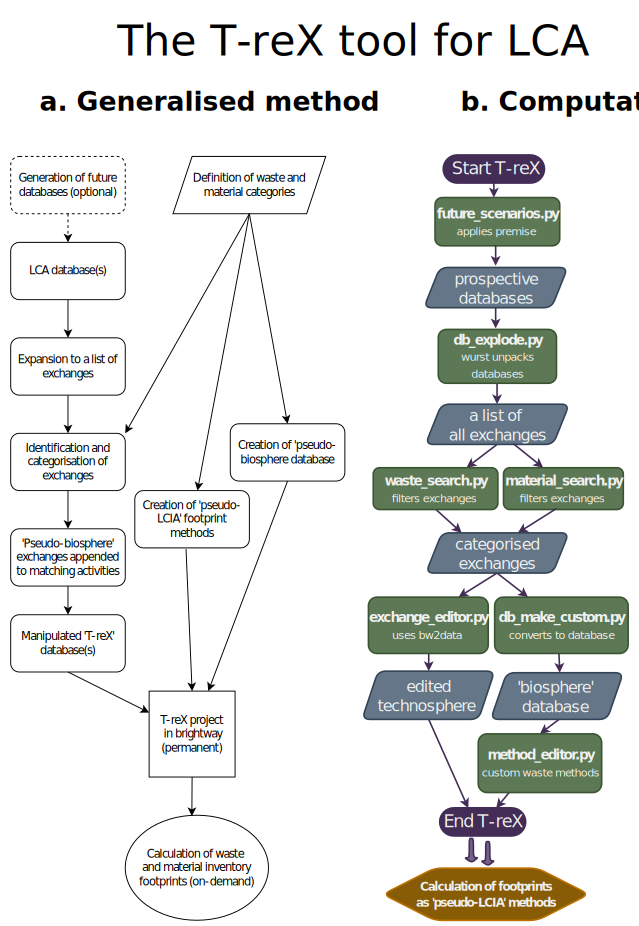
\includegraphics[width=0.5\linewidth]{figures/T-reX_method.pdf}
    \label{fig:methods-flowchart}
\end{figure}


\subsection{Case Study Methodology}\label{sec:method-case_study}

We investigated five types of Li-ion batteries, each represented by specific market activities:
\begin{itemize}[itemsep=0pt]
    \item Li-ion, NMC111, rechargeable, prismatic
    \item Li-ion, LiMn2O4, rechargeable, prismatic
    \item Li-ion, NCA, rechargeable, prismatic
    \item Li-ion, NMC811, rechargeable, prismatic
    \item Li-ion, LFP, rechargeable, prismatic
\end{itemize}

In addition to the waste and material inventory footprint methods created by the T-reX tool, the following standard LCIA methods were applied for comparison:

\begin{itemize}[itemsep=0pt]
    \item ReCiPe 2016 v1.03, midpoint (I)
    \item EF v3.0 no LT
    \item EDIP 2003 no LT
    \item Crustal Scarcity
\end{itemize}

The primary source of life cycle inventory data for this case study was ecoinvent 3.9.1 cutoff. Additionally, the T-reX tool was used to create prospective database sets using the \mbox{REMIND} model with the following Representative Concentration Pathways (RCPs):
\begin{itemize}
    \item SSP2-base: representing an approximate 3.5°C increase in global temperatures to 2100
    \item SSP2-PkBudg500: representing the achievement of Paris climate goals, ca. 1.3°C increase to 2100
\end{itemize}

For each pathway, databases were created with texttt{premise}~\citep{sacchi2022premise} and processed with the T-reX tool over the time series: 2020, 2040, 2060, 2080, 2100.

\subsubsection{Calculations}
For each combination of activity, method, and database, a single score `LCIA' was calculated along with details of the top contributing processes. Additionally, for the Waste and Material Footprint methods, a contribution analysis was performed. This involved utilizing the \texttt{bwa.compare\_activities\_by\_grouped\_leaves} function from the \texttt{brightway2\_analyzer} package~\citep{mutel2016brightway2analyzer}, an additional component of the Brightway2 LCA framework. This function performs graph traversal on the impact matrix of the LCA object to a specified cutoff and groups the resulting leaves by their CPC codes. This provides insight into the products and sectors in the supply chain of the activity that carry the most responsibility for the final footprint.




\section{Results}
\cbox{Section word count: 1400}
\label{sec:results}
\cbox{Section word count: 1800}

\subsection{WasteAndMaterialFootprint tool}\label{sec:results-wmf}
We have written an extension to the brightway2 LCA framework that calculates the waste footprint of a product or service.
It finds upstream waste flows in a supply chain, categorises waste flows into 14 types and finds hotspots in waste generation.
It explodes the database, identifies upstream waste exchanges, edits them and writes custom WasteFootprint methods. The waste flows then become pseudo-biosphere flows and the waste footprint can be calculated as an LCIA method. The WasteFootprint tool can be easily applied to calculate the `footprints' of other supply-chain flows such as water, gas, and critical raw materials.

In the context of environmental impact assessments, where a variety of indicators have been proposed and debated for their significance and communicability \citep{vanham2019footprints,ridoutt2013footprints}, the WasteAndMaterialFootprint (WMF) tool serves to re-simplify environmental decision-making. This tool leverages the findings that a limited set of indicators can cover a significant portion of environmental impact variance \citep{steinmann2017resourcefootprints}, enabling more streamlined and effective assessment processes.

\subsubsection{Waste exchanges}\label{sec:results-wmf-waste_exchanges}

In LCA waste flows are not considered as fundamental biosphere exchanges, but rather as technosphere flows. Waste produced by an activity is transferred to a relevant waste treatment activity where it is accepted `burden-free' and transformed into a combination of emissions and other waste `products'~\citep{guinee2021wasteisnotaservice}. There can be several treatment steps in this pathway leading, ultimately, to a mass of material being deposited in a landfill. In this system of waste accounting, the impacts apportioned to the waste-producing activity are a sum of those incurred by the transport, treatment, and final disposal of the waste into terrestrial or aquatic environments. In particular, the extensive work of~\cite{doka2024publications} has contributed significantly to understanding the environmental impacts of waste treatment processes and the long-term impacts of disposal. 

The purpose of the WMF tool is not to quantify the environmental impacts of waste treatment, but rather to quantify the waste flows themselves, even those that are finally consumed by waste treatment processes. It provides, thus, not an impact assessment in the traditional sense, but an accounting of the waste generated by a product or service, regardless of the end-of-life fate of these flows. By definition, the development of the `circular economy' necessitates the reduction and ultimate elimination of waste---though whether this objective is thermodynamically impossible has long been the subject of lively debate by~\cite{ayres1998recycling},~\cite{reuter2012recyclinglimits} and many others. In any case, waste avoidance is of critical importance and by quantifying and classifying the waste total attributed to a product or service in an LCA database, the WMF tool provides a practical means to identify hotspots and opportunities for waste reduction and efficiency.

The logic of screening for waste exchanges is based on a set of boolean search queries (`AND', `OR', and `NOT') that are applied in a list comprehension to the names of every exchange in the LCA database (see `search\_queries.py' for the full list). In this way, the search queries enable classification into categories (such as `hazardous solid' and `incineration liquid') and permit the identification of waste exchanges in addition to those directly connected to waste treatment processes. The search queries are tailored to the specific database and the user can easily modify them to suit their needs. In the default settings, there are a total of 18 waste classifications (9 categories, each separated into liquid and solid waste) For example, the identification of `non-hazardous solid' waste exchanges is based on the following search query; \texttt{AND = [`waste'], NOT = [`hazardous', `radioactive'], UNIT = [`kilogram']} (this can also be inferred and confirmed by comparison with the difference between the results of `total solid' and `hazardous solid').\ \autoref{tab:wf_results} presents a list of waste exchanges identified in the prospective database built from `ecoinvent 3.9.1' according to the IAM model `REMIND' with the RCP `PkBudg500' in the year 2100. Note that for prospective databases, a waste category for `carbon dioxide' has been created to account for the carbon capture and storage (CCS) that has been implemented in this model. 

\begin{table}[ht]
    \centering
    \caption{WasteFootprint search results for the database `ecoinvent cutoff 3.9.1, REMIND, SSP2, PkBudg500, 2100'.}\label{tab:wf_results}
    \begin{tabular}{llr}
        \toprule
        \textbf{Waste exchanges} & \textbf{Unit} & \textbf{Exchange count} \\
        \midrule
        digestion & kilogram & 4 \\
        composting & kilogram & 26 \\
        open burning & kilogram & 535 \\
        incineration & kilogram & 2171 \\
        recycling & kilogram & 137 \\
        landfill & kilogram & 1530 \\
        hazardous & kilogram & 1928 \\
        carbon dioxide & kilogram & 119 \\
        total & kilogram & 29524 \\
        digestion & cubic meter & 16 \\
        composting & cubic meter & 0 \\
        open burning & cubic meter & 0 \\
        incineration & cubic meter & 2 \\
        recycling & cubic meter & 0 \\
        landfill & cubic meter & 2 \\
        hazardous & cubic meter & 437 \\
        carbon dioxide & cubic meter & 0 \\
        total & cubic meter & 4360 \\
        \bottomrule
\end{tabular}
\end{table}

\subsubsection{Material exchanges}\label{sec:results-wmf-material_exchanges}

The logic for the identification of material exchanges with the WMF tool differs from that used to identify waste exchanges in that the search queries are based on the names of the so-called relevant `market activities' for the material of interest. That is, for material $x$, all exchanges with the name `market for material $x$' are identified and subsequently apportioned a (`pseudo-biosphere') material demand exchange of the same sign and magnitude as the original exchange. A useful feature of the WMF tool is that, in cases where there are several markets for one material or material group, the program can easily aggregate these exchanges. For example, exchanges with markets for the rare-earth-elements (REEs) `market for cerium', `market for dysprosium', `market for erbium', etc.\ can be aggregated into a single indicator category for REEs. Similarly, the total demand for all critical raw materials (CRMs) can be easily calculated in the same manner. 

As discussed in the introduction~\ref{sec:introduction} there are some existing material demand methods in the standard LCIA method sets, including the `crustal scarcity indicator' (which provides only an aggregated, abstracted endpoint)~\citep{arvidsson2020csi} and the (deprecated) EDIP 2003 material use indicators (which provide endpoints in fundamental units)~\citep{hauschild2003edip}. In these methods, the material demand is calculated based on the total mass that is extracted from the environment, thus, their focus is essentially solely on the mining-related exchanges that bring these materials from the biosphere into the technosphere. In the WMF tool, however, the accounting for material demand is based on exchanges solely within the technosphere. This offers a different perspective, allowing for the estimation of overall supply-chain material demands that consider the entire life cycle of an activity, including non-direct impacts on the market such as co-production of other materials. Consider a demand for an activity containing a metal, for example; while the existing material use methods allow one to calculate the total mass of that metal that is extracted from the environment, the WMF tool can provide insight into the broader supply-chain impacts of the demand for this metal. If the production other materials are attributed to the production of this metal, these would appear as negative material demands in the WMF results---supply chain pressure for one material can result in lessening of supply chain pressure for another. In the results of the Li-ion battery case study in \autoref{sec:results-case_study}, we will see that this is indeed the case for the demand for nickel, which, because of such effects, is counter-intuitively negative despite the presence of nickel in the final products.


\subsection{Case study: Li-ion batteries}\label{sec:results-case_study}


As listed in \autoref{sec:method-case_study}, this case study calculated the waste and material footprints (as well as a variety of other indicators) for the unaltered inventories for five Li-ion batteries with the functional unit being 1~kg of battery. The purpose of this simple case study was to test, verify, and demonstrate the functionality and limitations of the WMF tool. This section includes some highlights of the results and the full results are available in the supplementary material.

\subsubsection{Temporal and scenario variation in waste and material footprints}\label{sec:results-case_study-total_footprints}

\autoref{fig:waste_total} shows the total solid waste footprint for the five Li-ion batteries in the case study from 2020 to 2100 under the SSP2 scenario using the baseline and PkBudg500 RCPs of the REMIND model. The NMC811 battery has the largest footprint, producing over 50~kg of waste per kilogram of battery produced. The LiMn2O4 battery has the smallest footprint, producing less than 4~kg of waste per kilogram of battery. In each case there was a slight downward trend in the waste footprints between 2020 and 2100. This is most notable in the period between 2020 and 2040 and is attributable to the relatively rapid decrease in fossil-fuel use that is included in the models over this time. For the total waste generated by these batteries, there was very little difference observed between the baseline and PkBudg500 RCPs.


\begin{figure}[ht!]
    \centering
    \includegraphics[width=\linewidth]{figures/total_waste.png}
    \caption{Total solid waste footprints for the five Li-ion batteries in the case study from 2020 to 2100 under the SSP2 scenario using the baseline and PkBudg500 RCPs of the REMIND model.}\label{fig:waste_total}
\end{figure}

The inclusion of carbon capture and storage in the prospective databases using the PkBudg500 RCP is evident in \autoref{fig:carbondioxide}, which shows a rapid increase in the production of carbon dioxide `waste' over the period from 2020--2040 that is not seen in the baseline.


\begin{figure}[ht!]
    \centering
    \includegraphics[width=\linewidth]{figures/carbondioxide.png}
    \caption{Carbon dioxide waste (from carbon capture and storage) footprints for the five Li-ion batteries in the case study from 2020 to 2100 under the SSP2 scenario using the baseline and PkBudg500 RCPs of the REMIND model.}\label{fig:carbondioxide}
\end{figure}

For the phosphate demand footprints that are depicted in \autoref{fig:phosphate}, the LFP (lithium iron phosphate) battery has a much larger footprint than the other batteries, consistent with its composition. In this case, the phosphate footprint of all batteries is shown to decrease over the period from 2020--2100, and the RCP scenarios are seen to converge between 2020 and 2040.

\begin{figure}[ht!]
    \centering
    \includegraphics[width=\linewidth]{figures/phosphate.png}
    \caption{Phosphate material demand footprints for the five Li-ion batteries in the case study from 2020 to 2100 under the SSP2 scenario using the baseline and PkBudg500 RCPs of the REMIND model.}\label{fig:phosphate}
\end{figure}

\subsubsection{Contribution of `top-processes' in the supply chain}\label{sec:results-case_study-topprocesses}

\autoref{fig:top_contribution} shows the contribution of the `top-processes' to the cobalt footprint of the LiMn2O4 battery under the baseline scenario from 2020--2100. The total footprint is seen to almost triple, from 2.2~kg/kg in 2020 to 6.2~kg/kg in 2100. This result is likely a reflection of the electrification of the transport sector that is included in the REMIND model. The fractional contributions of the top processes is remains relatively steady over the coming century in this case. 

\begin{figure}[ht!]
    \centering
    \includegraphics[width=0.8\linewidth]{figures/top-processes.png}
    \caption{Contribution of `top-processes' to the case study from 2020 to 2100 under the SSP2 scenario using the baseline and PkBudg500 RCPs of the REMIND model.}\label{fig:top_contribution}
\end{figure}

\subsubsection{Contribution of industrial sectors in the supply chain}\label{sec:results-case_study-topsectors}

\autoref{fig:cpc_contribution} shows the contribution of industrial sectors (grouped by CPC classifications) to the total liquid waste footprint of the NCA battery under the PkBudg500 pathway.

\begin{figure}
    \centering
    \includegraphics[width=0.8\linewidth]{figures/cpc_contribution.png
    }
    \caption{Contribution of industrial sectors to the liquid waste footprint of the NCA battery from 2020 to 2100 under the SSP2 scenario using the PkBudg500 RCP of the REMIND model.}\label{fig:cpc_contribution}
\end{figure}

\section{Discussion}
\label{sec:discussion}
Given that waste generation and material demand are often strongly associated with the environmental impacts of human activities~\citep{laurenti2023wastefootprint,steinmann2017resourcefootprints, demirer2019wastefootprint}, we consider it of high importance that they are included LCA accounting. Although there are existing LCIA methods that provide endpoint impact scores related to material demand and waste generation, they generally contain convoluted formulae or subjective weighting, or their complexity and lack of transparency can make them difficult to use and interpret~\citep{foen2021ecofactors,hauschild2003edip,cen2019en15804, arvidsson2020csi,foen2021ecofactors}.

T-reX advances the state-of-the-art in LCA providing practitioners with a simple, flexible, and transparent way to calculate supply chain waste and material footprints, delivering results in standard units and as direct aggregations of the relevant demand inventories. Once LCA databases in the \texttt{brightway} project have been processed with T-reX, the user can easily apply the T-reX `pseudo-LCIA' methods to calculate the waste and material inventory footprints in the same way that they would with a conventional LCIA method.

The simple case study of five Li-ion batteries presented in this paper demonstrated the  utility, flexibility as well as some limitations of T-reX.

First, by adjusting the user configuration for future scenarios and waste/material categorisation we produced a set of customised versions of current and prospective ecoinvent databases along with a `pseudo-biosphere' T-reX database. Then, by applying the T-reX `pseudo-LCIA' methods, categorised waste and material inventory footprints for a number of present and future supply chains were trivial to calculate. Additionally, visual exploration in \texttt{ActivityBrowser} was possible because the T-reX `pseudo-LCIA' methods are integrated within the \texttt{brightway} project in the same way as standard LCIA methods.

One current limitation of T-reX is that it does not yet provide specific information (in a readily accessible format) on the composition of the waste generated. This is the information that would be needed to thoroughly assess the potential environmental impacts of this waste. Currently, the user would need to manually explore the waste footprint inventory produced by the application of the T-reX to determine if the waste generated represents an actual loss of resources or environmental risk, or, for example, is simply a transfer of the `overburden' in mining activity, which is classified as `inert waste'. A methodic classification of waste exchanges and the end-of-life fates is expected to be facilitated by the ever more detailed and disaggregated data that is seen in each successive release of ecoinvent~\citep{fitzgerald2023ecoinventdocumentation}.

The utility of T-reX in studies of future supply chains is limited by the fact that the currently available prospective databases focus largely on changes in the energy, steel, cement, and transport sectors~\citep{sacchi2023premisedocs}. As demonstrated in the results of the case study---where there was often very little scenario-temporal change in many waste and material footprint indicators---the utility of prospective LCA is restricted if there is inadequate adaption of the future background inventories. In particular, the inclusion of scenarios with future waste processing technology could greatly improve our predictions of waste and material flows and offer valuable insight into their potential impacts~\citep{bisinella2024wastelca}. A strong focus on enhancing these prospective databases is, thus, of critical importance to the future of prospective LCA, and by extension, to the development of the `circular economy'. 

\cbox{Section word count: 450}

\section{Conclusions}
\label{sec:conclusions}
\cbox{Section word count: 250}
We have written the T-reX tool, an extension to the brightway2 LCA framework that enables the user to calculate the waste and material footprints of a product or service in an LCA database. It explodes the database, identifies upstream waste and material exchanges, edits them, and writes matching custom WMF methods. These exchanges become pseudo-biosphere flows and thus, the footprint can be calculated as with the existing LCIA methods. The WMF tool can be easily customised by the user to calculate the footprints of other supply-chain flows such as water, gas, and critical raw materials.

This paper extends the state of knowledge by exploring the relationship between various waste aggregation methods and environmental damage indicators, contributing to a deeper understanding of life cycle waste inventories and their association with supply-chain risk and potential environmental damage.


% Back matter
\section*{Data availability} 
All data used in this analysis are publicly available online under the noted sources. The T-reX tool is installable via the Python Package Index (PyPI) and is available at \url{https://pypi.org/project/T-reX}.
The full source code for the T-reX tool is available at \url{https://www.github.com/Stew-McD/T-reX}.
A user guide and comprehensive documentation are available at \url{https://T-reX.readthedocs.io}.

\section*{CRediT authorship contribution statement}
\cbox{Co-authors, please check this and change as necessary.}
\textbf{Stewart Charles McDowall:} Methodology, Software, Validation, Formal analysis, Investigation, Data curation, Writing - original draft, Writing - review \& editing, Visualization.
\textbf{Elizabeth Lanphear:} Conceptualization, Methodology, Software, Validation, Writing - review \& editing.
\textbf{Stefano Cucurachi:} Conceptualization, Writing - review \& editing, Supervision, Project administration, Funding acquisition.
\textbf{Carlos Felipe Blanco:} Conceptualization, Writing - review \& editing, Supervision, Project administration, Funding acquisition.

\subsection*{Alternative CRediT statement}

\includegraphics[width=\columnwidth, height=7cm, keepaspectratio]{credit.pdf}

\section*{Declaration of competing interest}
The authors declare that they have no known competing financial interests or personal relationships that could have appeared to influence the work reported in this paper.

\section*{Acknowledgements}
    Part of this research project was financially supported by the European Union's Horizon 2020 research and innovation programme under the grant agreement No. 101058522 (project FutuRaM --- futuram.eu). The authors would like to thank the reviewers for their valuable comments and suggestions.

\section*{Supplementary material}
    The supplementary material contains the following:
    \begin{enumerate}
        \item List of waste and material categories
        \item Example output of the T-reX tool
        \item List of identified waste and material exchanges
        \item Code (python script) used for case study
        \item Inventory and methods used in the case study
        \item Complete tabulated results of the case study
        \item Complete visualisations of the case study
    \end{enumerate}

\bibliographystyle{elsarticle-harv}
\bibliography{references.bib}
    
% \appendix


% \section{Example output}
% \label{app:example_output}

\end{document}